\begin{figure}[t]
    \centering
    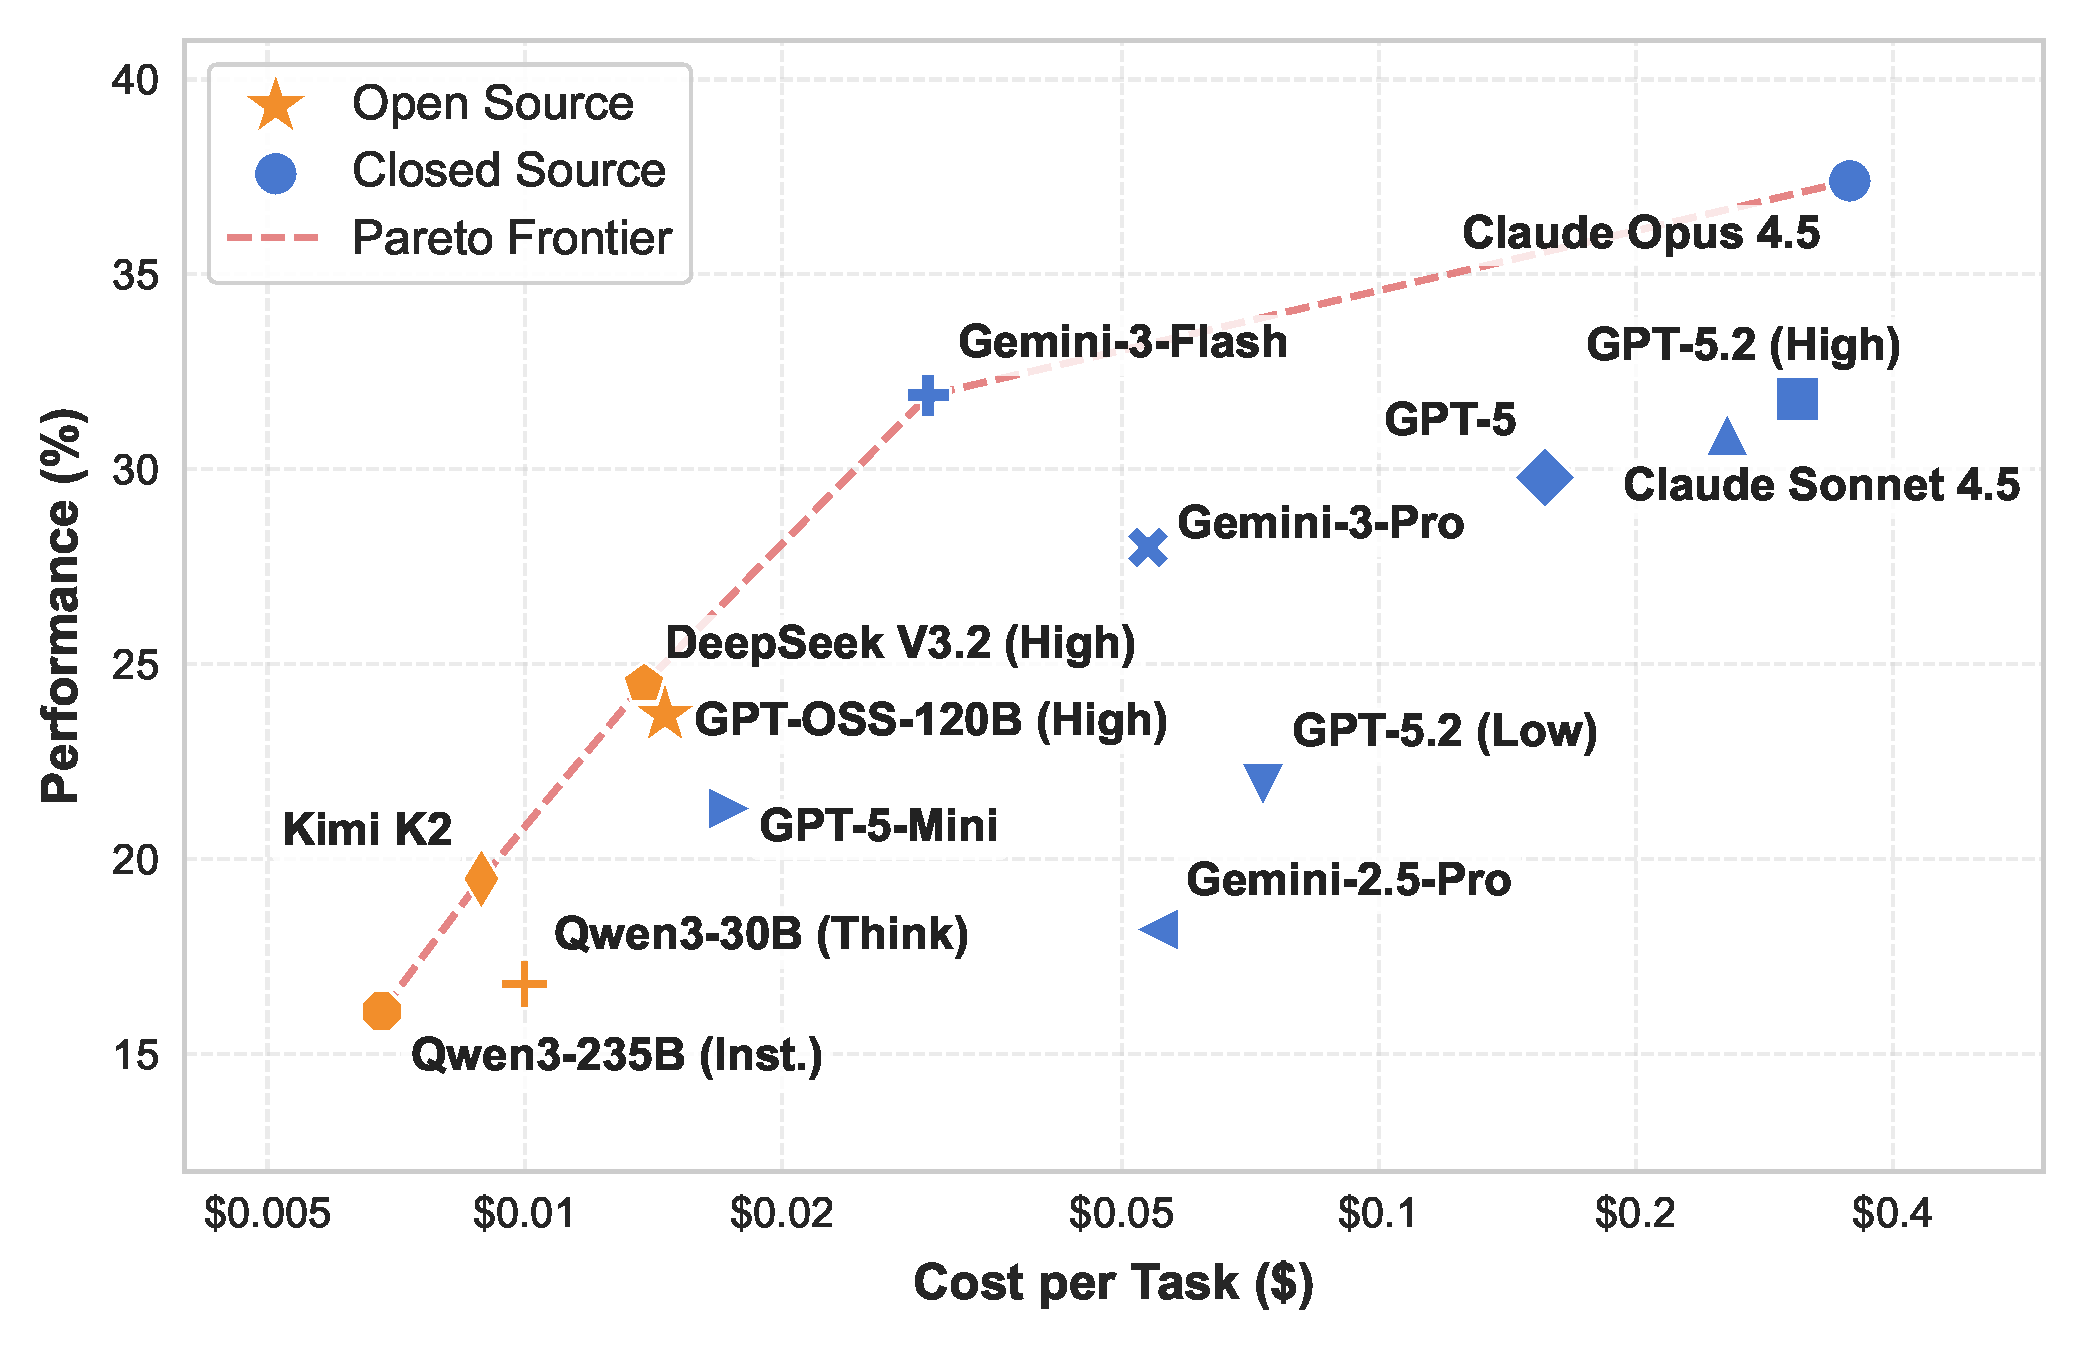
\includegraphics[width=1.0\linewidth]{figures/experiments/cost_vs_perf_new.pdf}
    \caption{\textbf{\ours{} 上智能体工具使用的性能--成本权衡。}图中给出闭源与开源模型的任务成功率及其单任务估算成本。开源模型成本更低，但成功率始终更低；成本较高的模型虽有适度性能增益，却仍远未达到可靠的任务完成水平。}
    \label{fig:cost_vs_preformance}
\end{figure}

\begin{figure*}[t]
 \centering
 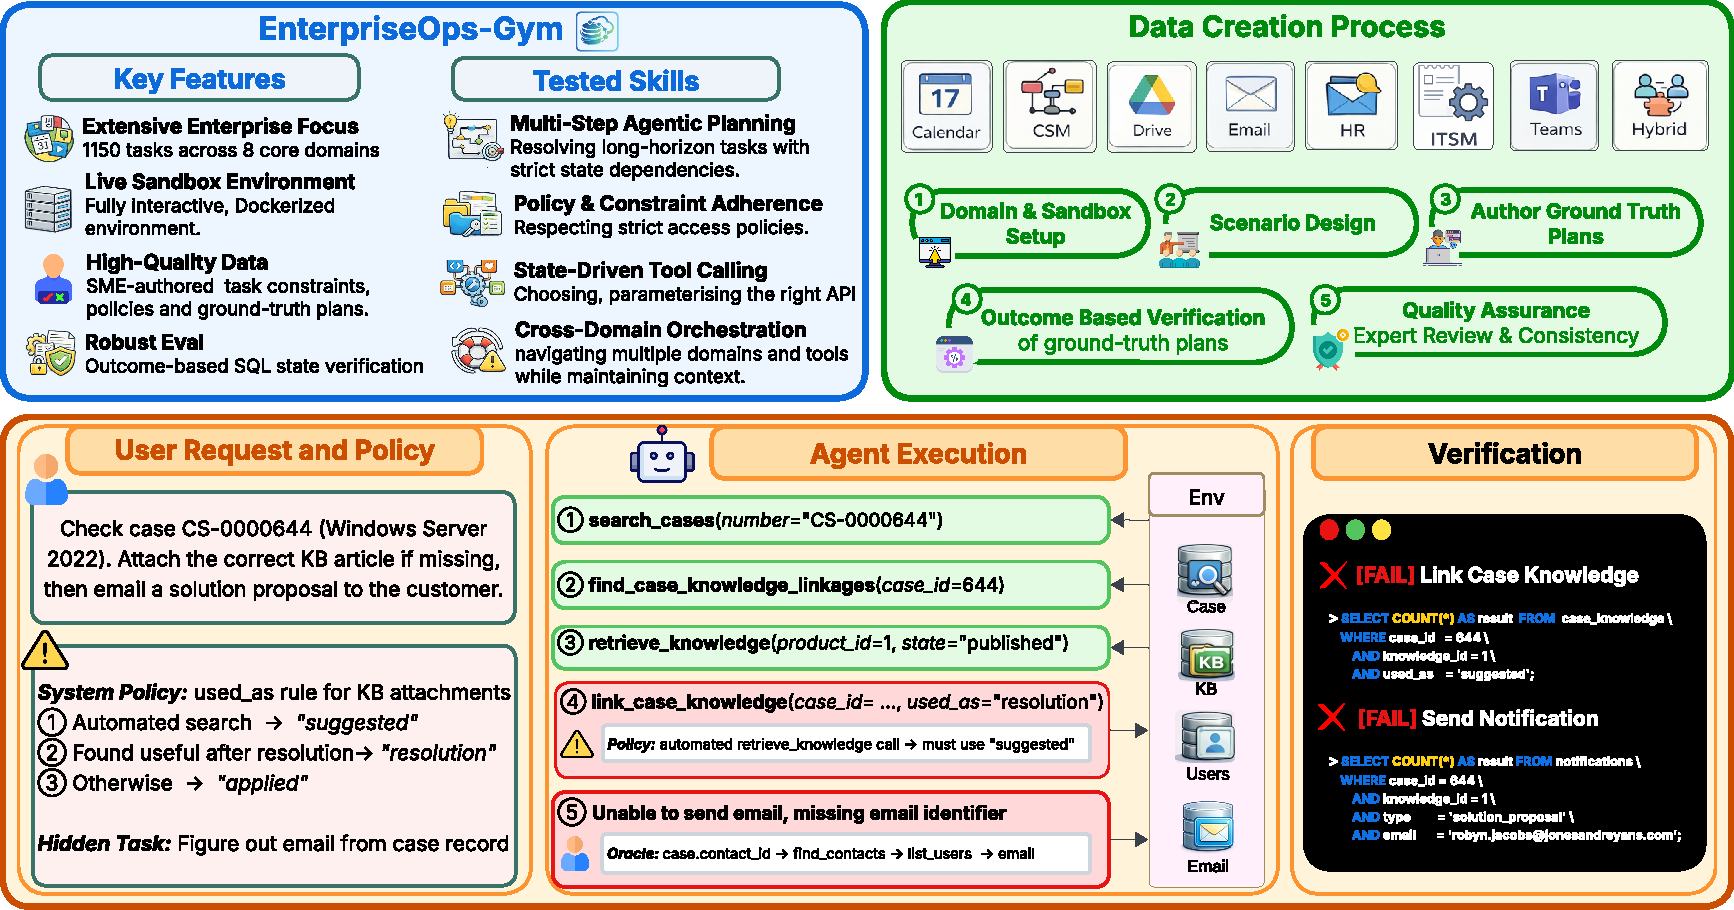
\includegraphics[width=1.0\linewidth]{figures/teaser_final.pdf}
 \caption{\textbf{\ours{} 概览：面向有状态智能体规划与工具使用的基准。}
（左上）\ours{} 覆盖八个企业领域，并在可复现沙箱中评估多步智能体规划、策略遵循、状态驱动工具调用与跨领域编排。
（右上）领域专家构建沙箱并编写贴近实际的单领域和跨领域任务，执行真值轨迹，编写以结果为中心的验证逻辑；经多阶段质量保证后，还为完成任务撰写人工专家计划。
（下方）给定任务及作为系统级策略的约束，智能体与环境交互并执行工具。最终状态验证器检查目标完成情况、策略合规性与副作用。图中示例里，智能体未遵守关联案例知识的系统策略：自动发现知识库时，必须将参数设为 ``suggested''；此外，它还因未解析给定案例的标识符而没有正确发送邮件通知。}
 \label{fig:gym_teaser}
\end{figure*}

\section{引言}

如今，大语言模型最常被部署为对话助手，用来回答问题、起草邮件和概括文档~\citep{openai2025gpt5, anthropic2025sonnet45}。但一种影响更为深远的能力正在快速出现：LLM 作为代表用户行动的\textit{自治智能体}~\citep{xu2024theagentcompanybenchmarkingllmagents}。设想一个智能体只根据一条指令，就能检索网页上的实时库存信息、找出最佳产品并完成购买，无需任何后续输入。规划和工具使用的近期进展，正使\textit{AI 员工}的愿景越来越可信：自治智能体可处理从软件工程~\citep{jimenez2024swebench}、数据分析~\citep{workarena2024}到销售运营和企业管理~\citep{huang-etal-2025-crmarena, huang-etal-2025-crmarena-pro}的专业工作流。然而，要在现实的专业部署中有效运作，这类智能体不能只会遵循指令；它们还必须：（1）在交错的长工具调用序列中连贯地维护状态；（2）执行跨越数十个动作的多步计划；（3）严格遵从工作场所的访问控制策略和流程规则。

这些要求在企业领域尤为关键。在这里，智能体不只是检索信息；它们会直接修改在线数据库、触发下游工作流，并影响真实用户。动作带有状态且往往不可逆；错误会在相互连接的系统中悄然传播；严格的组织策略约束着每一步。图~\ref{fig:gym_teaser} 展示了一个此类任务：用户任务与细致的系统策略约束相互作用，所需能力远不止表层的指令跟随。智能体既要完成搜索案例、检索知识库文章、通知客户这样的多步工作流，也要遵守知识库文章标记的三级策略，并通过串联多个工具独立解析一项隐含信息，即客户的电子邮件地址。同样重要的是，智能体还必须知道何时停止。盲目尝试违反策略的任务会破坏系统状态，在生产环境中带来直接的安全风险。

尽管这一挑战迫在眉睫，现有基准仍未能充分刻画它。通用工具使用评测~\citep{li-etal-2023-api, qin2024toolllm, chen2025acebenchwinsmatchpoint} 将工具调用视为原子且无状态的操作，衡量的是没有状态依赖或跨系统协调的短序列准确率。面向企业的基准~\citep{workarena2024, boisvert2024workarenacompositionalplanningreasoningbased, huang-etal-2025-crmarena, huang-etal-2025-crmarena-pro, jha2025itbenchevaluatingaiagents, vishwakarma2025llmshelpworksandbox} 已出现，以应对专业环境中的挑战。它们虽作出了重要贡献，却通常局限于单一厂商生态（例如仅 Salesforce 或仅 ServiceNow），环境较浅，数据库表少于 25 张、工具不足 50 个、任务跨度较短，且对智能体行为的策略约束有限（见表~\ref{tab:related_works_comparison}）。

为弥补这一缺口，我们提出 \textbf{\ours{}}，一个用于在高保真企业仿真中评估智能体规划的基准。\ours{} 横跨八个相互连接的生态系统，既包括 Calendar、Drive、Teams 和 Email 等通用生产力工具，也包括人力资源（HR）、IT 服务管理（ITSM）、客户服务管理（CSM）等关键业务功能，并由需要协调跨领域执行的 Hybrid 类别统一起来。该基准在这些领域上包含 1,150 个由专家编写的任务，其中 30 个不可行场景用于检验智能体能否正确拒绝无法满足的请求，同时不在系统中留下副作用。任务由手写 SQL 脚本验证，检查目标完成、状态完整性、策略合规性和非预期副作用。\ours{} 运行于完全交互式的容器化环境，其中包含 164 张关系数据库表和 512 个功能工具；专家轨迹平均为 9 步，最长达 34 步。这样的规模旨在压力测试企业自动化的核心挑战：长程规划、跨系统状态管理与受策略约束的执行。

我们对 14 个前沿模型的评估揭示了当前智能体能力与企业要求之间的显著鸿沟。性能高度受领域复杂度影响：模型在协作任务上表现最好，顶尖模型在 Email、Teams 和 Drive 上达到 51--52\%，但在受策略管控的 ITSM（28.5\%）和跨领域 Hybrid 任务（30.7\%）上明显下降。这些恰恰是不可避免需要约束感知推理的领域。总体最佳模型 Claude Opus~4.5 仅达到 37.4\%，开源模型进一步落后。不可行性识别是关键弱点，即使最佳模型也只能在 53.9\% 的策略违规任务上干净地拒绝。测试时计算扩展有所帮助，却不是普遍的补救方案：某些工作流很早进入平台期，或者无论思考预算如何增加都只得到有限改进。重要的是，我们发现战略性规划而非工具使用才是主要瓶颈：加入干扰工具几乎没有影响，而提供人工编写的计划可使模型提升 14--35 个百分点。更复杂的多智能体编排同样无法弥合这个差距；由于任务具有很强的顺序状态依赖，把任务拆解为子任务甚至会使性能回退。综上，当前智能体尚未准备好用于自治企业部署。

本文贡献如下：
\begin{itemize}
    \item 我们提出 \ours{}：一个覆盖八个企业领域、含 1,150 个专家策划任务的基准。它以结果为中心的验证机制约束目标完成、状态完整性、策略合规性和副作用检查，并包含 30 个不可行任务，用于评估安全拒绝行为。
    \item 我们构建了一个完全交互式、容器化的企业环境，含 164 张关系数据库表和 512 个功能工具，复杂度比先前企业基准高一个数量级。
    \item 我们评估了 14 个前沿模型，揭示并分析规划、状态管理与策略合规方面的系统性失败模式，并给出构建更可靠企业智能体的可操作洞见。我们还将向社区发布 \ours{}，以推动有状态智能体规划与企业工具使用研究。
\end{itemize}
